\documentclass[a4paper,11pt]{article}
\usepackage[T1]{fontenc}
\usepackage[utf8]{inputenc}
\usepackage{lmodern}

\usepackage{makeidx}
    % Needed to build the index.

\usepackage{amsmath}
    % Brings the align environment for lining up equations on the =.

\usepackage{amssymb}
    % For the number set symbols.

\usepackage{cancel}
    % For striking out bits of equations that simplify.

\usepackage{graphicx}
    % Can't have pictures/photos/figures from files without that.
    % Note that vanilla latex will only accept eps.
    
\usepackage{subfigure}
    % Lets me have labels such as a) b) c) inside a figure environment.

\usepackage[font=footnotesize, labelfont=bf]{caption}
    % So that I can add long captions under figures.
    % It provides me with \caption* that does not appear in the list of
    % figures but formats the text like \caption does.  It also lets me
    % use line breaks in the caption, and even bullet/enumerated lists.

\usepackage{color}
    % For rendering text is eps_tex files produced by InkScape, even
    % if the text is black.

\usepackage{booktabs}
    % For professional-looking tables.
    % Brings the \toprule, \midrule and \bottomrule.
    % Remember not to use vertical rules in tables: they look cheap.

\usepackage[version=3]{mhchem}
    % For chemical formulas.
    % Brings \ce.ormulas.

\usepackage[mediumspace,mediumqspace,squaren]{SIunits}
    % Otherwise I can't write the mu symbol for micrometers.
    % It also brings me the \degree symbol, woo!
    % No decibel though, I need to make this one myself.

\usepackage{stmaryrd}
    % For the llbracket and rrbracket to denote integer intervals.

\usepackage{varioref}
    % For fancier references that also tell the page number.
    
\usepackage{todonotes}
    % Big post-its, handy while writing.
    
\usepackage[]{biblatex}
    % Fantastic bibliography manager that I'll use just for its
    % \citetitle command.

\newcommand{\decibel}{dB}
\newcommand{\equaldef}{\stackrel{\text{\tiny def}}{=}}
\newcommand{\transp}{^T}
\newcommand{\norm}[1]{\left\| #1 \right\|}
\newcommand{\abs}[1]{\left| #1 \right|}

\graphicspath{{./figures/}}
\addbibresource{bibliography.bib}

\title{}
\author{}

\begin{document}

\maketitle
%\tableofcontents

\begin{abstract}
\end{abstract}





%=============================================================================

\section{Introduction}
HIFI \cite{AA_518_L6} on the HSO \cite{AA_518_L1}.
Built to do such and such science [REFERENCE].
Works on this principle (heterodyne, therefore coherent).
Coherence allows for interferences.
Interferences give rise to standing waves.
Standing waves modulate the coupling of the backend to the LO, the sky and the calibration black bodies.
If the calibration ignores the standing waves, then the result has error bars that can easily dominate all the other sources of uncertainty, as shown on figure~\ref{fig:scatter_real_data}.

\begin{figure}
    \centering
    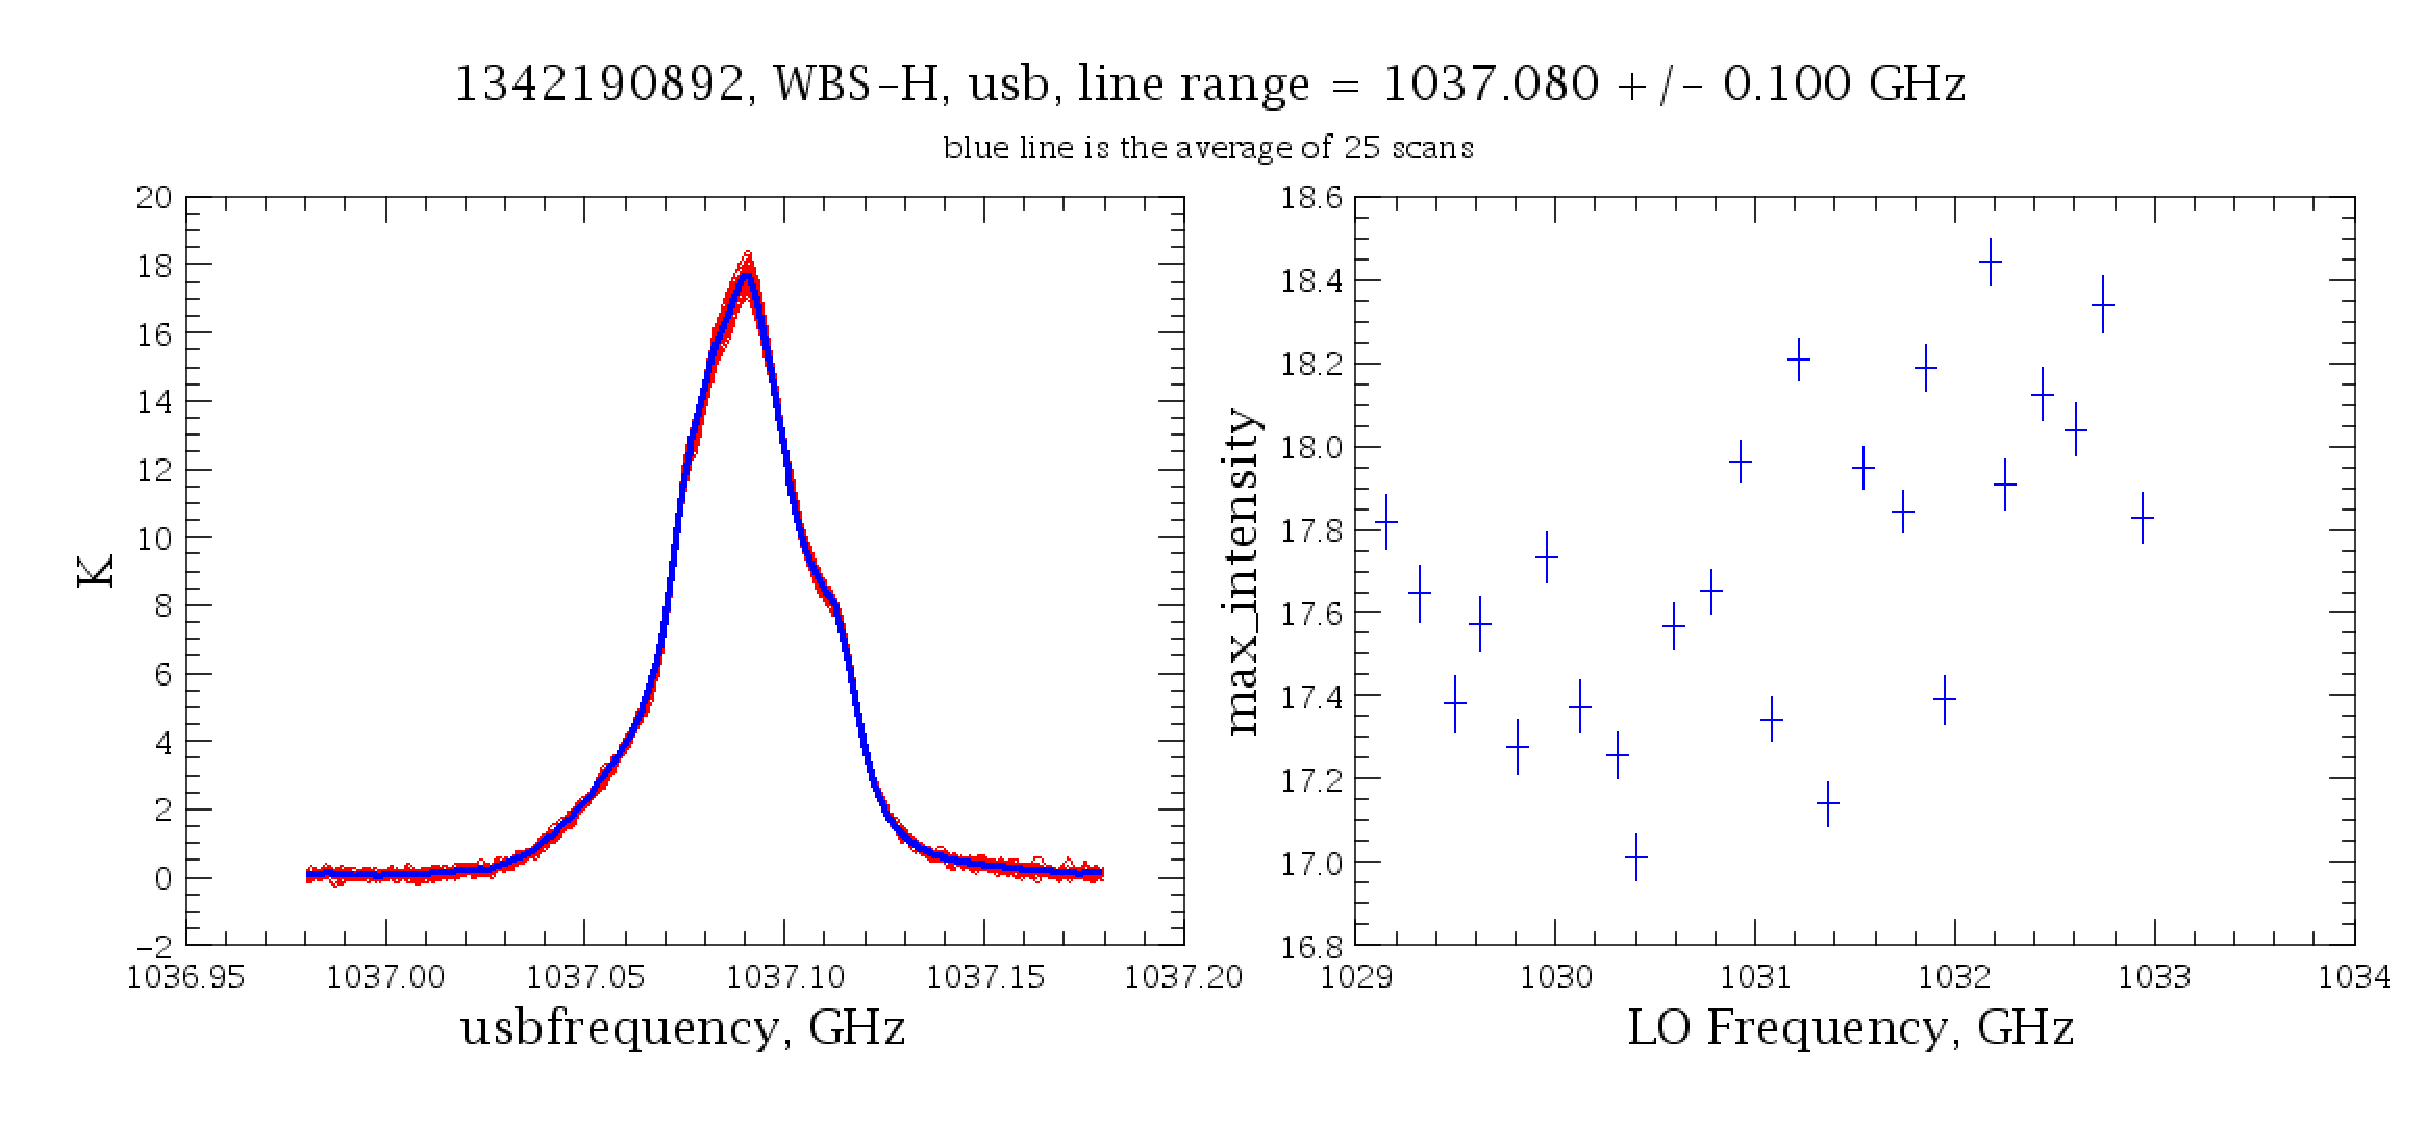
\includegraphics[width=\textwidth]{1342190892_4a_line_frequency_1037-080GHz_level_usb_20_WBS-H_max_intensity}
    \caption{\label{fig:scatter_real_data}The same line observed at 25 different LO frequencies.  If there were no standing waves, all the red curves (left plot) would overlap and there would be no scatter of the peak intensity (right plot).  Standing waves modulate the gain of the system, and the current calibration scheme ignores them.}
\end{figure}





%=============================================================================

\section{Modeling standing waves}



%-----------------------------------------------------------------------------

\subsection{Principle}

Jones matrices capture the idea of transfering energy from one polarization to another \cite{hecht2002optics}.
Note that they cannot handle non-polarized light.
This is not a problem for us as wire grid polarizers ensure that everything in our system is polarized (linearly or elliptically).
They traditionally work in 2D but it is trivial to extend them to work in 3D.

Scattering matrices \cite{siegman1986lasers} capture the idea of transfering energy from one side (port) of an optical element (network) to another.

Putting 3D Jones matrices inside scattering matrices is a natural way of doing both the port-to-port and the polarization energy transfer at the same time.

A system like HIFI is made of a few dozens of networks.
All these networks interact together, two by two, since there exist at least one optical path between each pair or networks.
The number of interactions in the system increases with the square of the number of networks.

We propose a method to reduce the number of networks without losing any information.
Our model computes the scattering matrix of the network equivalent to the whole system.
Then, knowing how the system reacts to an input is merely a matter of multipling the scattering matrix of the network equivalent to the whole system with a vector of inputs to get a vector of outputs.

As shown of figure~\ref{fig:cascading}, two networks A and B connected by one port (port $\alpha$ for A and port $\beta$ for B) can be seen as a single equivalent  network C.
The scattering matrix of that equivalent network takes into account the infinite reflections between the two original networks.
\begin{figure}[hbtp]
    \centering
    \input{figures/cascading.eps_tex}
    \caption{\label{fig:cascading}Two networks P and Q connected by one port have an equivalent network S.}
\end{figure}

If we have a method to compute an equivalent network, then we can apply it recursively to an entire system to get the network equivalent to the whole system.
This is illustrated by figure~\ref{fig:cascading_example}
\begin{figure}[hbtp]
    \centering
    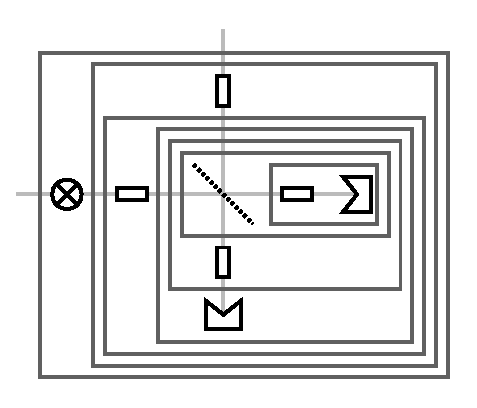
\includegraphics{cascading_example}
    \caption{\label{fig:cascading_example}}
\end{figure}

Not iterative; it's a one-pass solver that directly gives the steady state.

%-----------------------------------------------------------------------------

\subsection{Simplifications}

The frequency regime suggests that we should use quasi optics to properly account for the diffraction of the beams.
However, this complicates things a lot, and therefore we simplified the problem.
$\Rightarrow$ Plane waves, single mode.

Plane wave isn't bad anyway since we put all our networks at the waists of the beams, where the wave front is flat.

The discrepencies due to these simplifications can be abstracted by parameters in our model.
For example, if a higher mode does not couple to a mixer, then its power is --for all practical purpose-- lost, and therefore a term of loss can model it.

%-----------------------------------------------------------------------------

\subsection{Elements of modeling}
\paragraph{Chaining networks.}
\begin{figure}[hbtp]
    \centering
    \input{figures/combining_networks.eps_tex}
    \caption{\label{fig:between_networks}
        Notations used to describe two networks P and Q connected by one port.
        P~has $n_P$~ports and Q has $n_Q$~ports, here $n_P=4$ and $n_Q=3$;
        the equivalent network S has $n_S = n_P + n_Q - 2$ ports, here $n_S=5$.
        We use a common indexing scheme for the scattering matrices of P, Q and S:
        ports 1 to $n_P$ are ports of P (here 1 to 4),
        ports $n_P+1$ to $n_P+n_Q$ are ports of Q (here 5 to 7),
        ports 1 to $n_P+n_Q$ except $\alpha$ and $\beta$ are ports of S (here 1 to 7 except 3 and 5).
        The port~$\alpha$ of~P is connected to the port~$\beta$ of~Q, here $\alpha=3$ and $\beta=5$.
        Because of the connection, the output of port $\alpha$, $b_\alpha$, is equal to the input of port $\beta$ noted $a_\beta$; we name it $c$.  Likewise, we name $d$ the output of $\beta$ which is equal to the input of $\alpha$.
        The scattering matrices of P, Q and S are noted $P$, $Q$ and $S$.
        }
\end{figure}
Figure~\ref{fig:between_networks} expands on figure~\ref{fig:cascading} to introduce notations useful for describing mathematically what happens to the electric field between two connected networks.
In order to simplify the reasoning and shorten the equations, we use an indexing system that is common to $P$, $Q$ and $S$.  This means that the way we index our matrices is unconventional: the matrix $Q$ is indexed by port numbers ranging from $n_P+1$ to $n_P + n_Q$, therefore $Q_{1, j}$ does not exist since the port 1 does not belong to Q.  In order to write a software implementation of these equations, one level of indirection is required to transform the port numbers into conventional matrix indices.
Finally, the elements of the matrices $P$, $Q$ and $S$ are themselves matrices: they are Jones matrices.

Equation~\eqref{eq:between_networks} decribes the electric field between P and Q once the steady state is established.
\begin{equation}
    \left\lbrace
    \begin{aligned}
        c
        &=
        P_{\alpha, \alpha} d + \sum_{j = 1 \atop j \neq \alpha}^{n_P}
        \left(
            P_{\alpha, j}a_j
        \right)
        \\
        d
        &=
        Q_{\beta, \beta} c + \sum_{j = n_P+1 \atop j \neq \beta}^{n_P + n_Q}
        \left(
            Q_{\beta, j}a_j
        \right)
    \end{aligned}
    \right.
    \label{eq:between_networks}
\end{equation}
In equation~\eqref{eq:between_networks}, $c$~and~$d$ depend on each other.
Equation~\eqref{eq:d} presents the solution of this system for~$d$.
\begin{equation}
    d =
    (I - Q_{\beta, \beta} P_{\alpha, \alpha})^{-1}
    \left[
        Q_{\beta, \beta}
        \sum_{j = 1 \atop j \neq \alpha}^{n_P}
        \left(
            P_{\alpha, j}
            a_j
        \right)
        +
        \sum_{j = n_P \atop j \neq \beta}^{n_P + n_Q}
        \left(
            Q_{\beta, j}
            a_j
        \right)
    \right]
    \label{eq:d}
\end{equation}
In equation~\eqref{eq:d}, $I$ represents the identity matrix that matches the size of $Q_{\beta, \beta}P_{\alpha, \alpha}$ (that is, 3--by--3 as these are 3D Jones matrices).
We are certain that $I - Q_{\beta, \beta} P_{\alpha, \alpha}$ has an inverse because the system has losses: if it did not have an inverse then the system could store an infinite amount of energy and therefore never reach a steady state, this system would not be physical.
Since~$d$ is an input for~P, we can express the outputs of P in terms of~$d$.
\begin{gather}
\begin{aligned}
    \forall i, i
    &\in
    \left\llbracket 1 ; n_P \right\rrbracket, i \neq \alpha
    &
    b_i
    &=
    P_{i, \alpha} d
    + \sum_{j = 1 \atop j \neq \alpha}^{n_P}
    \left(
        P_{i, j}a_j
    \right)
\end{aligned}
\notag
\\
\begin{aligned}
    b_i
    &=
        \sum_{j = 1 \atop j \neq \alpha}^{n_P}
        \left[
            \left(
                P_{i, \alpha}
                (I - Q_{\beta, \beta} P_{\alpha, \alpha})^{-1}
                Q_{\beta, \beta}
                P_{\alpha, j}
                +
                P_{i, j}
            \right)
            a_j
        \right]
    \\
    &+
        \sum_{j = n_P+1 \atop j \neq \beta}^{n_P + n_Q}
        \left[
            \left(
                P_{i, \alpha}
                (I - Q_{\beta, \beta} P_{\alpha, \alpha})^{-1}
                Q_{\beta, j}
            \right)
            a_j
        \right]
\end{aligned}
\label{eq:P_side_of_S}
\end{gather}
Equation~\ref{eq:P_side_of_S} gives us what we are looking for: the ouputs~$b_i$ as functions of the inputs~$a_j$.
It is however limited to what we can call the ``P-side'' of the equivalent network S: the output ports~$b_1$ to~$b_{n_P}$.
We repeat this reasoning with~$c$ and~$Q$ to get~$b_i$ for the ``Q-side'' of the equivalent network S: outputs~$b_{n_P}$ to~$b_{n_P+n_Q}$.

We have expressed the elements of~$b$ as a linear combinations of the elements of~$a$,
therefore we have all the coefficients~$S_{i, j}$ of the matrix of our equivalent network.
This matrix is divided into four sections depending on the port numbers:
$i \in \llbracket 1 ; n_Q \rrbracket$ and
$i \in \llbracket n_P + 1 ; n_P + n_Q \rrbracket$,
and the same for~$j$ as shown in table \ref{table:equivalent_network}.
\begin{table}[htbp]
    \centering
    \begin{tabular}{r|c c}
        \toprule
            $S_{i, j}$
            &
            $j \in \llbracket 1 ; n_P \rrbracket$
            &
            $j \in \llbracket n_P + 1 ; n_P + n_Q \rrbracket$ \\
        \midrule
            $i \in \llbracket 1 ; n_P \rrbracket$
            &
            $
                P_{i, \alpha}
                R_P
                Q_{\beta, \beta}
                P_{\alpha, j}
                +
                P_{i, j}
            $
            &
            $
                P_{i, \alpha}
                R_P
                Q_{\beta, j}
            $
            \\
            $i \in \llbracket n_P + 1 ; n_P + n_Q \rrbracket$
            &
            $
                Q_{i, \beta}
                R_Q
                P_{\alpha, j}
            $
            &
            $
                Q_{i, \beta}
                R_Q
                P_{\alpha, \alpha}
                Q_{\beta, j}
                +
                Q_{i, j}
            $
            \\
        \bottomrule
    \end{tabular}
    \caption{\label{table:equivalent_network}S-parameters coefficients of the network S equivalent to P and Q connected by the ports~$\alpha$ (for P) and~$\beta$ (for Q) using a common indexing.}
    \caption*{
        Neither~$i$ nor~$j$ can take the values~$\alpha$ or~$\beta$: these two ports are hidden inside the equivalent network and are not accessible to the outside.

        $R_P = (I - Q_{\beta, \beta} P_{\alpha, \alpha})^{-1}$ and $R_Q = (I - P_{\alpha, \alpha} Q_{\beta, \beta})^{-1}$.
        These matrices correspond to the infinite reflections between the two networks P and Q, either seen from P or seen from Q.
    }
\end{table}

Table~\ref{table:equivalent_network} tells us how to compute the scattering matrix of a network S equivalent to two networks P and Q.
We can apply this method in order to recursively reduce the entire system, made of many networks arranged in a tree (in the graph theory sense of the word ``tree''), to one single network (Figure~\ref{fig:cascading_example}).
Calculating the response of a complex system to an input is then just a matter of multiplying its scattering matrix with an input vector.

\paragraph{Typical networks.}
Most are easy to model, at least at the first order.
Only the grids are really a pain.
\begin{itemize}
    \item Space: propagation changes the phase.
    \item Mirrors: they don't do much, just ignore them.
    \item Rooftop mirrors: these matter as they rotate polarization.
    \item Rectangular horns: at the first order, they transmit one linear polarization and reflect the other.
    \item Black bodies: weak reflection, scramble the polarization.
    \item Attenuator: reduces the amplitude.
    \item Grids: used Houde's work \cite{houde_2001}.
\end{itemize}

%=============================================================================

\section{Qualitative achievement}
Calibration paper: \cite{AA_537_A17}

The method described above allows us to compute the scattering matrix of a system provided we know the scattering matrices of the networks that constitute that systems.

Our test case is the HIFI spectrometer.
Its focal plane unit has many networks.


I put it all together to model the bands 3 and 4 of HIFI, which use martin puplet  interferometers (REFERENCE) to inject the LO and signal power with a minimum of loss.
These devices are nice because they allow you to get pretty much 100 percent of the incoming signal, but they come with a price: more reflections, therefore more standing waves.

I ran the model for different sources: the local oscillator, the sky on source, the sky off source, and the calibration black bodies.
Each simulation gave me a coupling spectrum.
I multiplied these couplings with a model of the radiation from the source (gaussian line), and the LO BB OFF sources (flat continuums).
Then I folded them simply, without using a physical model of the mixer, just by overlaping the LSB and USB.
Then I applied the calibration steps like HIFI does.

The result is visible on figure~\ref{fig:simulated_spectrum_dirty}.
The goal was to qualitatively replicate the observation presented in figure~\ref{fig:scatter_real_data}.
Even with rough guesses for the parameters, and the approximations we made, we do reproduce a scatter of the peak intensity of the line, with the right order.
\begin{figure}
    \centering
    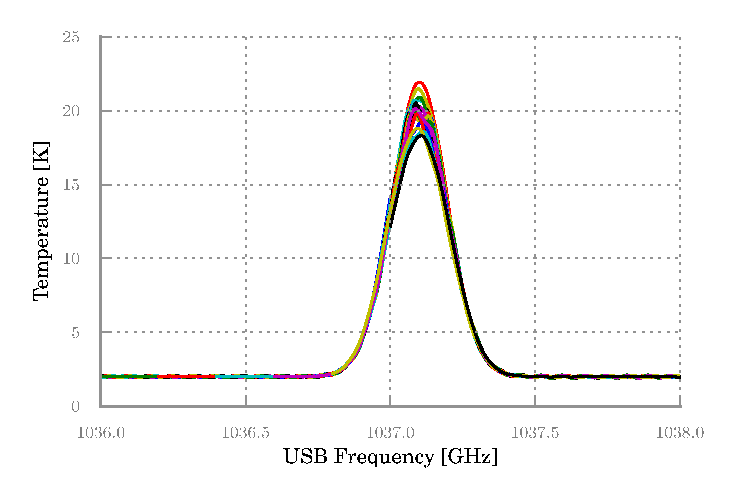
\includegraphics{bb-on_narrow}
    \caption{\label{fig:simulated_spectrum_dirty}Simulated spectra, the peak intensity varies because each LO tuning brings its own set of standing waves that modulates the coupling.}
\end{figure}

Our model gives us information that we do not get with real data: the sideband ratio.
The upper and lower sidebands are both modulated by standing waves, but they are modulated differently.
In a perfect system, the sideband ratio USB/(LSB+USB) is 0.5, but in reality it varies.
If we know the sideband ratio, then we can put it into the calibration equation in order to better calibrate the line or the continnuum intensity (one or the other).
Our model gives us access to the simulated sideband ratio, as shown on figure~\ref{fig:sbr}.
\begin{figure}
    \centering
    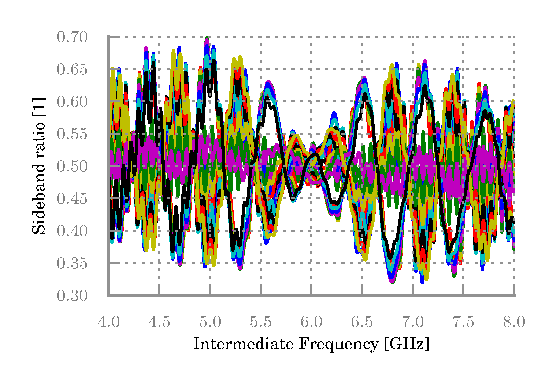
\includegraphics{sbr}
    \caption{\label{fig:sbr}Simulated sideband ratio}
\end{figure}

I recalibrated the spectrum to use the SBR information on the sky path; the result is shown in figure~\ref{fig:simulated_spectrum_corrected}.
It is better, but not perfect, because the SBR on the Black Body path is not taken into account.  If I make the black bodies really black, then the spectrum is perfect.
\begin{figure}
    \centering
    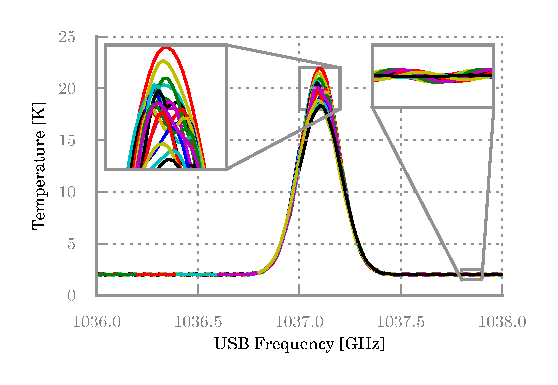
\includegraphics{bb-on_corrected-2}
    \caption{\label{fig:simulated_spectrum_corrected} Simulated spectrum, with calibration corrected for SBR on the sky, but not on the black bodies.  It's already better.  I can work a bit more on the calibration equation to clean it totally, because with non-reflective black bodies I get a perfectly corrected spectrum.}
\end{figure}





%=============================================================================

\section{Conclusion}
We have a way of modeling the interferences, and therefore the standing waves, in any coherent instrument.
The model produces results that are qualitatively consistent with many HIFI observations.
We showed that the model can give us information (notably the sideband ratio) that we can use to better calibrate data.
By modeling more acurately the networks, we are expecting to reproduce quantitatively HIFI data.
This would allow us to significantly reduce the incertainties in the calibration.

%=============================================================================

\printbibliography
\end{document}
